% !TeX root = main.tex
\chapter{СИСТЕМИЙН ХЭРЭГЖҮҮЛЭЛТ}

Энэ бүлэгт өмнөх бүлгүүдэд тодорхойлсон шаардлага, архитектур, өгөгдлийн загварт тулгуурлан боловсруулж дуусгасан дадал төлөвшүүлэх системийн хэрэгжүүлэлтийг тайлбарлана. Тодруулбал, системийг хэрэгжүүлэхэд ашигласан технологийн стек, кодын сангийн бүтэц, өгөгдлийн сангийн хэрэгжилт, домайн логикийн гол дүрмүүд, бэкэнд болон фронтэндийн үндсэн модулиуд, API-ийн зохион байгуулалт, хэрэглэгчийн интерфэйсийн шийдлүүд болон туршилтад бэлтгэсэн эцсийн боломжуудыг авч үзнэ.

Системийн эцсийн хувилбарт хэрэглэгч бүртгүүлэх, нэвтрэх, дадал үүсгэх, хуваарь болон олон төрлийн cue тохируулах, push notification хүлээн авах, гүйцэтгэл бүртгэх, ахицын статистик харах, дадлын хүчний оноо болон зөвлөмж авах, амжилт болон XP цуглуулах, санал хүсэлт болон судалгаанд оролцох зэрэг үндсэн урсгалууд бүрэн хэрэгжсэн. Иймээс энэ бүлэг нь 20 хэрэглэгчээр туршуулахад ашигласан бодит ажиллах хувилбарын хэрэгжүүлэлтийг нэгтгэн харуулна.

\section{Технологийн стек}

Эцсийн системийн хэрэгжүүлэлтэд ашигласан үндсэн технологиуд:

\begin{itemize}
  \item \textbf{Бэкэнд хүрээ:} NestJS v11 --- модульчилсан зохион байгуулалттай, REST API хөгжүүлэхэд тохиромжтой.
  \item \textbf{Хөгжүүлэлтийн хэл:} TypeScript --- статик төрлийн шалгалтаар кодын найдвартай байдлыг нэмэгдүүлсэн.
  \item \textbf{ORM ба миграц:} Prisma v7 --- схемд суурилсан өгөгдлийн загварчлал, миграцийн удирдлагыг хялбаршуулсан.
  \item \textbf{Өгөгдлийн сан:} PostgreSQL --- харилцаат өгөгдлийн бүтэцтэй системд найдвартай, өргөтгөх боломжтой.
  \item \textbf{Фронтэнд хүрээ:} React 18 + Vite --- компонентод суурилсан UI хөгжүүлэлт болон хурдан build.
  \item \textbf{Чиглүүлэлт:} React Router --- нэг хуудсын аппликэйшний дотоод чиглүүлэлтийг хэрэгжүүлсэн.
  \item \textbf{UI:} Tailwind CSS + shadcn/ui --- тогтвортой, дахин ашиглагдах интерфэйсийн хэв маяг.
  \item \textbf{Анимаци:} Framer Motion --- төлөвийн өөрчлөлтийг илүү ойлгомжтой харуулахад ашигласан.
  \item \textbf{Баталгаажуулалт:} JWT (Bearer token) --- stateless хандалтын хяналт хэрэгжүүлсэн.
\end{itemize}

Бэкэнд болон фронтэндийн аль аль нь TypeScript хэл дээр хэрэгжсэн нь өгөгдлийн бүтэц, enum, интерфэйсийн тодорхойлолтыг хоёр талд нийцтэй байлгах давуу талтай байв. Ингэснээр API-ийн гэрээний зөрчил, төрлийн алдааг хөгжүүлэлтийн шатанд илрүүлэх боломж нэмэгдсэн.

\section{Кодын сангийн бүтэц}

Системийг фронтэнд болон бэкэнд гэсэн хоёр үндсэн хэсэгт хуваан хэрэгжүүлсэн. Бэкэнд талд домайн логик, хэрэглээний үйлчилгээ, өгөгдөл хадгалах дэд бүтцийг ялган зохион байгуулсан бол фронтэнд талд дэлгэц, дахин ашиглах боломжтой компонент, API клиент, хэрэглэгчийн төлөвийг тусгаарласан бүтэц ашиглав.

\subsection{Бэкэндийн бүтэц}

Бэкэнд нь NestJS-ийн модульчилсан бүтэцтэй бөгөөд домайн дүрэм, хэрэглээний урсгал, өгөгдлийн түвшнийг ялгах зарчмыг баримталсан.

\begin{lstlisting}[language=bash, caption={Бэкэндийн директорийн бүтэц}]
backend/src/
  auth/           -- бүртгэл, нэвтрэлт, JWT баталгаажуулалт
  habits/         -- дадал үүсгэх, засах, архивлах, хуваарь
  progress/       -- гүйцэтгэл бүртгэх, ахицын тооцоолол
  reminders/      -- сануулгын үнэлгээ, үүсгэлт, үйлдэл
  analytics/      -- хэрэглээний идэвх, аналитик өгөгдөл
  domain/
    entities/     -- домайн объектууд
    enums/        -- enum тодорхойлолтууд
    repositories/ -- repository интерфэйсүүд
    rules/        -- stateless домайн дүрмүүд
  infrastructure/
    prisma/       -- Prisma-д суурилсан хэрэгжүүлэлт
\end{lstlisting}

\subsection{Фронтэндийн бүтэц}

Фронтэнд нь дэлгэц, UI компонент, API холболт, auth context, туслах сангууд гэсэн бүтэцтэйгээр зохион байгуулагдсан.

\begin{lstlisting}[language=bash, caption={Фронтэндийн директорийн бүтэц}]
frontend/src/
  pages/          -- үндсэн дэлгэцүүд
  components/     -- дахин ашиглагдах UI компонентууд
  api/            -- HTTP клиент ба endpoint функцууд
  lib/            -- theme, push notification, utility функцууд
  context/        -- auth болон ерөнхий төлвийн context
\end{lstlisting}

Ийм бүтэц нь хөгжүүлэлтийн явцад модулиудын хариуцлагыг тодорхой байлгах, цаашид өргөтгөх болон засварлах ажлыг хөнгөвчлөхөд чиглэсэн.

\section{Өгөгдлийн сангийн хэрэгжүүлэлт}

Өгөгдлийн сангийн бүтцийг Prisma ORM-ийн \texttt{schema.prisma} файлд тодорхойлж, PostgreSQL дээр миграцийн аргаар хэрэгжүүлсэн. Системийн төв өгөгдлийн нэгж нь \texttt{Habit} хүснэгт бөгөөд дадлын нэр, хэмжилтийн тохиргоо, эхлэх хугацаа, төлөв, сануулгын идэвхтэй эсэх зэрэг гол шинжүүдийг хадгална.

\begin{lstlisting}[language=SQL, caption={Дадлын үндсэн загвар}]
model Habit {
  id              String               @id @default(uuid())
  userId          String               @map("user_id")
  title           String
  measurementUnit String               @map("measurement_unit")
  targetValue     Float                @map("target_value")
  minimumTarget   Float                @map("minimum_target")
  startDate       DateTime             @map("start_date") @db.Date
  status          HabitLifecycleStatus @default(ACTIVE)
  reminderEnabled Boolean              @default(false)

  scheduleDays      HabitScheduleDay[]
  cues              HabitCue[]
  motivationProfile HabitMotivationProfile?
  logs              HabitLog[]
  reminders         Reminder[]
  srbaiAssessments  SrbaiAssessment[]
  reminderPolicy    ReminderPolicy?
}
\end{lstlisting}

Дадлын гүйцэтгэлийн бүртгэлийг хадгалах \texttt{HabitLog} загварт зөвхөн ``хийсэн'' эсэх төдийгүй, тухайн үйлдэл ямар нөхцөлд хийгдсэнийг илэрхийлэх \texttt{completionHour}, \texttt{coarseLocation}, \texttt{precedingRoutine} зэрэг талбаруудыг нэмж тодорхойлсон. Мөн гүйцэтгэлийн эх үүсвэрийг \texttt{CompletionTriggerSource} enum-аар ангилан хадгалдаг.

\begin{lstlisting}[language=SQL, caption={Гүйцэтгэлийн бүртгэлийн загвар}]
model HabitLog {
  status           HabitLogStatus
  actualValue      Float?
  completedAt      DateTime
  triggerSource    CompletionTriggerSource @default(UNKNOWN)
  linkedReminderId String?
  completionHour   Int?
  coarseLocation   String?
  precedingRoutine String?
}
\end{lstlisting}

Нийт 20 орчим үндсэн хүснэгт болон холбоос хүснэгтийг хэрэгжүүлсэн бөгөөд тэдгээрийн гол төлөөллийг Хүснэгт~\ref{tab:db-tables}-д нэгтгэн үзүүлэв.

\begin{table}[htbp]
\centering
\small
\setlength{\tabcolsep}{4pt}
\begin{tabular}{|p{4.2cm}|p{8.8cm}|}
\hline
\textbf{Хүснэгтийн нэр} & \textbf{Зорилго} \\ \hline
\texttt{users} & Хэрэглэгчийн бүртгэл, нэвтрэлтийн мэдээлэл \\ \hline
\texttt{habits} & Дадлын үндсэн мэдээлэл, хэмжилтийн тохиргоо \\ \hline
\texttt{habit\_steps} & Олон алхамтай дадлын жижиг алхмууд \\ \hline
\texttt{habit\_schedule\_days} & Дадлын идэвхтэй өдрүүдийн хуваарь \\ \hline
\texttt{habit\_cues} & Өдөөгч нөхцөлүүд: цаг, байршил, өмнөх үйлдэл \\ \hline
\texttt{habit\_motivation\_profiles} & Хувийн шалтгаан, зорилготой холбоотой мэдээлэл \\ \hline
\texttt{habit\_logs} & Гүйцэтгэлийн бүртгэл, нөхцөл байдлын агшин \\ \hline
\texttt{difficulty\_feedbacks} & Гүйцэтгэлийн дараах төвөгшлийн үнэлгээ \\ \hline
\texttt{reflections} & Эргэцүүлсэн санал, ашиг тусын тэмдэглэл \\ \hline
\texttt{reminders} & Илгээгдсэн сануулгын бүртгэл \\ \hline
\texttt{reminder\_actions} & Сануулгад өгсөн хэрэглэгчийн үйлдэл \\ \hline
\texttt{reminder\_policies} & Сануулгыг аажмаар бууруулах бодлогын төлөв \\ \hline
\texttt{srbai\_assessments} & SRBAI үнэлгээний асуулгын хариулт, оноо \\ \hline
\texttt{user\_activity\_logs} & Аппликэйшний ерөнхий хэрэглээний идэвхийн бүртгэл \\ \hline
\texttt{adaptation\_recommendations} & Ахиц болон дадлын хүчнээс үүссэн зөвлөмжүүд \\ \hline
\texttt{article\_interactions} & Суралцах агуулгатай хийсэн хэрэглэгчийн харилцан үйлчлэл \\ \hline
\texttt{push\_subscriptions} & Web push notification илгээх төхөөрөмжийн subscription мэдээлэл \\ \hline
\texttt{user\_badges} & Хэрэглэгчийн нээсэн амжилт, badge мэдээлэл \\ \hline
\texttt{user\_feedbacks} & Аппын түвшний санал хүсэлт, алдааны мэдэгдэл \\ \hline
\end{tabular}
\caption{Өгөгдлийн сангийн үндсэн хүснэгтүүд}
\label{tab:db-tables}
\end{table}

Ийнхүү өгөгдлийн сангийн бүтэц нь хэрэглэгчийн дадлыг зөвхөн бүртгэх бус, харин сануулга, нөхцөл байдал, автоматжилт, ахицын шинжилгээ зэрэг зан үйлийн талаарх мэдээллийг хадгалах боломжтой болсон.

\section{Домайн логикийн хэрэгжүүлэлт}

Энэхүү системийн онцлог нь гол зан үйлийн дэмжлэгийн логикийг энгийн CRUD үйлдлээс ялган, тусдаа домайн дүрмийн түвшинд хэрэгжүүлсэнд оршино. Сануулга өгөх эсэхийг шийдэх, дадлын хүчийг тооцоолох, дасан зохицох зөвлөмж гаргах зэрэг нь stateless дүрмийн хэлбэрээр боловсруулагдсан.

\subsection{Сануулгын шийдвэрийн дүрэм}

\texttt{ReminderDecisionRules} нь тухайн мөчид сануулга үүсгэх эсэхийг шийдвэрлэнэ. Энэхүү дүрэм нь дараах үндсэн шалгууруудыг авч үздэг.

\begin{itemize}
    \item тухайн дадалд сануулга идэвхтэй эсэх;
    \item өнөөдөр хуваарьт өдөр мөн эсэх;
    \item идэвхтэй cue байгаа эсэх.
\end{itemize}

Дээрх нөхцөлийг шалгасны үндсэн дээр \texttt{SHOULD\_REMIND}, \texttt{REMINDER\_DISABLED}, \texttt{NOT\_SCHEDULED\_TODAY}, \texttt{NO\_ACTIVE\_CUES} зэрэг шалтгаануудын аль нэгээр шийдвэр гаргана.

\begin{lstlisting}[language=JavaScript, caption={Сануулгын шийдвэрийн дүрэм}]
export class ReminderDecisionRules {
  static decide(input: ReminderDecisionInput): ReminderDecisionResult {
    const isScheduledToday =
      CueScheduleRules.isScheduledToday(input.scheduleDays);
    const activeCues = CueScheduleRules.getActiveCues(input.cues);
    const activeCueCount = activeCues.length;

    let reason: ReminderDecisionReason;

    if (!input.reminderEnabled) {
      reason = ReminderDecisionReason.REMINDER_DISABLED;
    } else if (!isScheduledToday) {
      reason = ReminderDecisionReason.NOT_SCHEDULED_TODAY;
    } else if (activeCueCount === 0) {
      reason = ReminderDecisionReason.NO_ACTIVE_CUES;
    } else {
      reason = ReminderDecisionReason.SHOULD_REMIND;
    }

    return {
      shouldRemind: reason === ReminderDecisionReason.SHOULD_REMIND,
      reason,
      isScheduledToday,
      activeCueCount,
      evaluatedAt: new Date().toISOString(),
    };
  }
}
\end{lstlisting}

Сануулга үүсгэх үед давхардсан илгээлтээс сэргийлэхийн тулд \texttt{ReminderExecutionService}-д нэг цагийн bucket бүхий cooldown механизм ашигласан. Өөрөөр хэлбэл, ижил дадалд нэг цагийн хүрээнд олон ижил сануулга үүсэхээс хамгаална.

\subsection{Дадлын хүчний тооцоолол}

\texttt{HabitStrengthRules} нь дадлын хүчийг илэрхийлэх хэд хэдэн зан үйлийн үзүүлэлтийг тооцоолдог. Үүнд:

\begin{itemize}
    \item гүйцэтгэлийн хувь;
    \item өөрийн санаачилгатай гүйцэтгэлийн хувь;
    \item гүйцэтгэлийн тогтвортой байдал;
    \item нөхцөл байдлын тогтвортой байдал.
\end{itemize}

\subsubsection*{SRBAI-ийн оноо}

SRBAI-ийн 4 асуултын хариултаас дундаж түүхий оноог гаргаж, үүнийг 0--100 хооронд нормчилсон.

\begin{lstlisting}[language=JavaScript, caption={SRBAI-ийн оноо тооцоолох дүрэм}]
static scoreSrbai(input: SrbaiScoreInput): SrbaiScoreResult {
  const rawAverage =
    (input.item1 + input.item2 + input.item3 + input.item4) / 4;

  const normalizedScore100 =
    Math.round(((rawAverage - 1) / 6) * 10000) / 100;

  return { rawAverage, normalizedScore100 };
}
\end{lstlisting}

\subsubsection*{Нөхцөл байдлын тогтвортой байдал}

Сүүлийн гүйцэтгэлийн бүртгэлүүдэд тулгуурлан гүйцэтгэлийн цаг, ерөнхий байршил, өмнөх үйлдлийн давтамжийн хэв маягийг шинжилж, modal rate-ийн аргаар нөхцөл байдлын тогтвортой байдлыг тооцоолно.

\begin{lstlisting}[language=JavaScript, caption={Нөхцөл байдлын тогтвортой байдлын тооцоолол}]
static computeContextStability(snapshots: Array<{
  completionHour: number | null;
  coarseLocation: string | null;
  precedingRoutine: string | null;
}>): number {
  const n = snapshots.length;
  if (n === 0) return 0;

  const modalRate = (values: Array<string | number | null>): number | null => {
    const valid = values.filter(v => v !== null);
    if (valid.length === 0) return null;
    const freq = new Map<string | number, number>();
    for (const v of valid) freq.set(v, (freq.get(v) ?? 0) + 1);
    const maxCount = Math.max(...freq.values());
    return maxCount / n;
  };

  const rates = [
    modalRate(snapshots.map(s => s.completionHour)),
    modalRate(snapshots.map(s => s.coarseLocation)),
    modalRate(snapshots.map(s => s.precedingRoutine)),
  ].filter((r): r is number => r !== null);

  if (rates.length === 0) return 0;
  const avg = rates.reduce((a, b) => a + b, 0) / rates.length;
  return Math.round(avg * 100 * 100) / 100;
}
\end{lstlisting}

\subsubsection*{Нийлмэл дадлын хүчний оноо}

Судалгааны хүрээнд дадлын хүчийг дараах нийлмэл томьёогоор үнэлсэн.

\[
HS = 0.60 \times SRBAI_{100} + 0.25 \times Consistency_{100} + 0.15 \times ContextStability_{100}
\]

Эцсийн оноог дараах түвшинд ангилна.

\begin{itemize}
    \item 0--39: сул;
    \item 40--69: хөгжиж буй;
    \item 70--100: хүчтэй.
\end{itemize}

\begin{lstlisting}[language=JavaScript, caption={Нийлмэл дадлын хүчний онооны дүрэм}]
static computeCompositeScore(input: CompositeScoreInput): CompositeScoreResult {
  const finalScore = Math.round(
    (0.60 * input.srbaiScore
    + 0.25 * input.consistencyScore
    + 0.15 * input.contextStabilityScore) * 100) / 100;

  let stage: CompositeStage;
  if (finalScore < 40)      stage = CompositeStage.WEAK;
  else if (finalScore < 70) stage = CompositeStage.BUILDING;
  else                      stage = CompositeStage.STRONG;

  return { ...input, finalScore, stage, evaluatedAt: new Date().toISOString() };
}
\end{lstlisting}

\subsection{Дасан зохицох зөвлөмжийн дүрэм}

\texttt{AdaptationRules} нь гүйцэтгэлийн хувь, сануулгаас хамааралтай байдал, өөрийн санаачилгатай гүйцэтгэл, дадлын хүчний оноо, сүүлийн төвөгшлийн үнэлгээ зэрэг үзүүлэлтүүдэд үндэслэн зөвлөмж гаргана. Эцсийн хэрэгжүүлэлтэд дараах үндсэн анхаарлын чиглэлүүдийг тодорхойлсон.

\begin{itemize}
    \item \textit{reduce\_reminders};
    \item \textit{maintain};
    \item \textit{increase\_support};
    \item \textit{review\_difficulty};
    \item \textit{celebrate\_consistency}.
\end{itemize}

Мөн 7, 21, 66 удаагийн гүйцэтгэлийн үе шаттай уялдуулан ахицын баяр тэмдэглэлийн мессеж үүсгэх логикийг оруулсан.

\section{Бэкэнд модулиудын хэрэгжүүлэлт}

\subsection{Бүртгэл ба хандалтын модуль}

Хэрэглэгчийн бүртгэл, нэвтрэлтийг JWT-д суурилсан байдлаар хэрэгжүүлсэн. Нууц үгийг \texttt{bcrypt} ашиглан hash хэлбэрээр хадгалдаг. Нэвтэрсний дараа хэрэглэгч Bearer token авч, хамгаалагдсан endpoint-ууд руу хандах боломжтой болно. Мөн хэрэглэгч зөвхөн өөрийн \texttt{userId}-тай холбоотой өгөгдөлд хандах хязгаарлалтыг сервер талд шалгадаг.

\subsection{Дадлын удирдлагын модуль}

Энэ модуль нь дадал үүсгэх, засах, архивлах, жагсаалт авах, өнөөдрийн хуваарьт дадлуудыг шүүх зэрэг үндсэн боломжуудыг агуулна. Дадлын хэмжилтийн тохиргоо, хуваарь, өдөөгч нөхцөл, хувийн шалтгаан зэрэг мэдээллийг тусдаа хүснэгтүүдэд хадгалдаг ч хэрэглэгчийн хувьд нэг логик бүтэн урсгал байдлаар ажиллана.

\texttt{GET /users/:userId/habits/today} endpoint нь тухайн өдрийн идэвхтэй хуваарьт дадлуудыг буцааж, интерфэйсийн үндсэн дэлгэцэд өнөөдрийн хийх ёстой дадлуудыг харуулахад ашиглагдана.

\subsection{Ахицын модуль}

Ахицын модуль нь гүйцэтгэл бүртгэх, бодит утгыг minimum target болон target value-тай харьцуулан үнэлэх, ахицын summary гаргах үүрэгтэй. Гүйцэтгэлийг бүртгэх үед \texttt{metMinimum}, \texttt{metTarget} зэрэг үзүүлэлтийг автоматаар тооцоолж хадгална.

Мөн progress summary түвшинд дараах мэдээллүүдийг нэгтгэн гаргах байдлаар хэрэгжүүлсэн.

\begin{itemize}
    \item гүйцэтгэлийн хувь;
    \item өөрийн санаачилгатай гүйцэтгэлийн хувь;
    \item сануулгаас хамааралтай гүйцэтгэлийн хувь;
    \item ахицын хандлага;
    \item сүүлийн бүртгэлийн тойм.
\end{itemize}

\subsection{Сануулгын модуль}

Сануулгын модуль нь системийн зан үйлд суурилсан логикийн хамгийн чухал хэсгүүдийн нэг бөгөөд дараах гурван түвшинд хэрэгжүүлсэн.

\begin{enumerate}
    \item \textbf{Шийдвэрийн түвшин} --- \texttt{ReminderDecisionRules} ашиглан сануулах эсэхийг тодорхойлох;
    \item \textbf{Гүйцэтгэлийн түвшин} --- \texttt{ReminderExecutionService} ашиглан сануулгыг бүртгэх, давхардлаас хамгаалах, хэрэглэгч рүү хүргэх;
    \item \textbf{Бодлогын түвшин} --- \texttt{ReminderPolicy} ашиглан дадлын хүч нэмэгдэхийн хэрээр сануулгын эрчмийг бууруулах.
\end{enumerate}

Сануулгад хэрэглэгч \texttt{DONE} эсвэл \texttt{SNOOZE} гэсэн хоёр үндсэн үйлдэл өгөх боломжтой. \texttt{DONE} тохиолдолд холбогдох гүйцэтгэлийн бүртгэл автоматаар үүсч, trigger source нь сануулгад тулгуурласан гэж тэмдэглэгдэнэ. \texttt{SNOOZE} тохиолдолд дахин сануулах хугацааг бүртгэнэ. Push notification дамжуулалтыг Web Push болон VAPID түлхүүрт суурилан хэрэгжүүлж, хэрэглэгчийн төхөөрөмжийн subscription мэдээллийг сервер талд хадгалсан. Мөн нийт хэрэглэгчдэд системийн мэдэгдэл хүргэх шаардлагад зориулан \texttt{ADMIN\_SECRET}-ээр хамгаалагдсан broadcast endpoint-ийг Swagger баримтжуулалттайгаар нэмсэн.

\subsection{Оролцооны болон урамшууллын модуль}

Хэрэглэгчийн идэвхийг нэмэгдүүлэх зорилгоор XP, badge, амжилтын мэдээллийг нэгтгэн буцаах \texttt{Engagement} модулийг хэрэгжүүлсэн. Тухайн хэрэглэгчийн нийт XP, нээсэн badge, идэвхтэй push subscription-ийн тоо зэрэг мэдээллийг \texttt{GET /users/:userId/engagement/summary} endpoint-оор фронтэндэд өгдөг. Амжилтын үндсэн төрлүүдэд анхны гүйцэтгэл, 7 болон 21 өдрийн дараалал, нийт 30 удаагийн гүйцэтгэл зэрэг milestone-уудыг оруулсан.

Мөн хэрэглэгч profile хэсгээс өөрийн нээсэн амжилтуудыг харах, амжилтын зураг болон текстийг бусад платформ руу хуваалцах боломжтой болсон. Энэ нь хэрэглэгчид ``хийсэн зүйлээ харах'' болон цааш үргэлжлүүлэх урам авах мэдрэмжийг өгөх зорилготой урамшууллын давхарга юм.

\section{Фронтэндийн хэрэгжүүлэлт}

Фронтэндийг React болон Vite ашиглан хэрэгжүүлсэн бөгөөд хөдөлгөөнт төхөөрөмж дээр ашиглахад тохиромжтой, PWA хэлбэрийн интерфэйсийг зорьсон. Интерфэйсийн зохиомжид энгийн байдал, хурдан бүртгэл, дадалтай холбоотой ахицын мэдээллийг ойлгомжтой харагдуулах зарчмыг баримталсан.

\subsection{Үндсэн дэлгэцүүд}

Фронтэндийн үндсэн дэлгэцүүдийг Хүснэгт~\ref{tab:frontend-screens}-д үзүүлэв.

\begin{table}[htbp]
\centering
\small
\setlength{\tabcolsep}{4pt}
\begin{tabular}{|p{3.8cm}|p{9.2cm}|}
\hline
\textbf{Дэлгэц} & \textbf{Гол функц} \\ \hline
Dashboard & Өдрийн идэвхтэй дадлуудын жагсаалт, хурдан бүртгэл, streak болон товч ахицын мэдээлэл \\ \hline
HabitDetail & Дадлын дэлгэрэнгүй, calendar түүх, бүх цагийн хүрээ, cue, шалтгаан, дадлын хүчний мэдээлэл \\ \hline
CreateHabit & Дадал үүсгэх/засах форм, хэмжилт, олон алхам, хуваарь, cue, шалтгаан, сануулгын тохиргоо \\ \hline
Reminders & Сануулгын жагсаалт, тайлбар, DONE/SNOOZE үйлдэл \\ \hline
Analytics & Ахицын шинжилгээ, calendar, heatmap, харьцуулсан үзүүлэлтүүд, зөвлөмж \\ \hline
Auth & Бүртгэл болон нэвтрэх дэлгэц \\ \hline
Profile & Theme, сануулгын зөвшөөрөл, амжилт, архив, санал хүсэлт, судалгааны холбоос \\ \hline
Learn & Зан үйлийн онолтой холбоотой сурах агуулгын хэсэг \\ \hline
\end{tabular}
\caption{Фронтэндийн үндсэн дэлгэцүүд}
\label{tab:frontend-screens}
\end{table}

Дашборд дэлгэц нь хэрэглэгчийн өдөр тутмын харилцааны гол цэг бөгөөд Зураг~\ref{fig:dashboard}-д харуулсан. Зүүн дэлгэц нь өнөөдрийн дадлуудыг гүйцэтгэлгүй буюу анхны байдлаар харуулж байгаа бол баруун дэлгэцэд нэгийг бүрэн, нэгийг хэсэгчлэн гүйцэтгэсэн байдал болон шинэ дадлын карт харагдаж байна.

\begin{figure}[htbp]
  \centering
  \begin{minipage}[b]{0.42\textwidth}
    \centering
    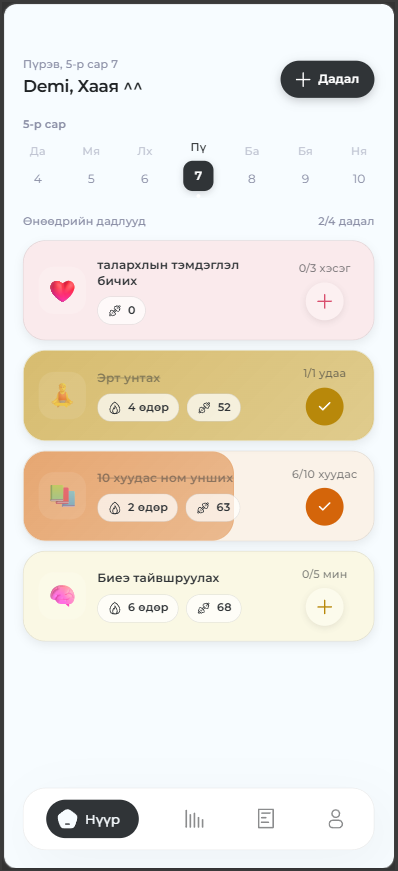
\includegraphics[width=\textwidth,height=0.46\textheight,keepaspectratio]{images/frontend/dashboard.png}
    \\[4pt]\small (а) Өдрийн дадлуудын жагсаалт
  \end{minipage}
  \hfill
  \begin{minipage}[b]{0.42\textwidth}
    \centering
    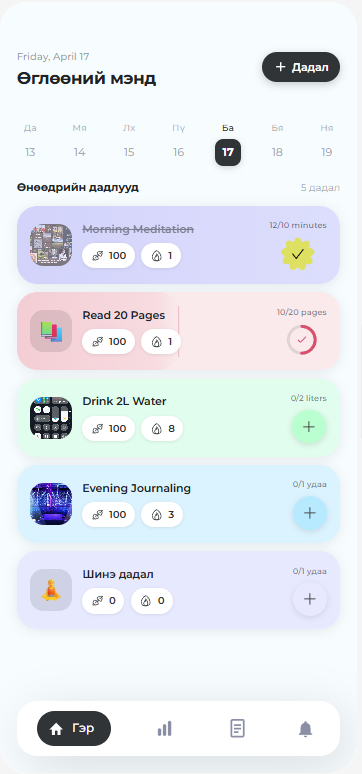
\includegraphics[width=\textwidth,height=0.46\textheight,keepaspectratio]{images/frontend/habitbutgesenDashboard.png}
    \\[4pt]\small (б) Зарим дадлуудыг гүйцэтгэсний дараа
  \end{minipage}
  \caption{Үндсэн (Dashboard) дэлгэц}
  \label{fig:dashboard}
\end{figure}

\subsection{Дадал үүсгэх дэлгэц}

Дадал үүсгэх интерфэйсийг ``Юу хийх вэ --- Хэзээ, ямар нөхцөлд хийх вэ --- Яагаад хийх вэ'' гэсэн гурван үндсэн ойлголтод тулгуурлан зохион байгуулсан. Ийм зохиомж нь олон салангид техникийн талбар бөглүүлэхээс илүү хэрэглэгчид ойлгомжтой урсгал бий болгох зорилготой.

Хэрэглэгч мэдээллээ оруулах үед дэлгэц дээр тухайн дадлын тодорхойлолт өгүүлбэр хэлбэрээр шууд бүрэлдэн харагдана. Өмнөх routine cue-ийн хувьд ``дараа'', ``өмнө'', ``үедээ'' гэсэн timing утгыг chip хэлбэрээр сонгох боломжтой бөгөөд сонгосон утга нь \texttt{precedingRoutine} талбарт кодлогдон хадгалагдаж, дадлын дэлгэрэнгүй болон notification мессежид зөв үгээрээ гарна. Мөн хэрэглэгч дадлыг хэмжигдэхүйц эсвэл хийсэн/хийгээгүй төрлөөр сонгох, олон алхам нэмэх, цагийн олон хүрээ, байршил, хуваарь, icon, өнгө, шалтгаан зэрэг мэдээллийг нэг урсгалаар тохируулах боломжтой болсон.

Дадал үүсгэх формын хоёр үндсэн хэсгийг Зураг~\ref{fig:addhabit}-д харуулав. Зүүн дэлгэц нь дадлын нэр, харагдах төрх, өгүүлбэрэн тодорхойлолт болон хуваарийн тохиргоог агуулж, баруун дэлгэцэд сануулгын идэвхжүүлэлт, цагийн хүрээ болон хэмжилтийн нарийвчлалтай тохиргоог харуулсан.

\begin{figure}[htbp]
  \centering
  \begin{minipage}[b]{0.42\textwidth}
    \centering
    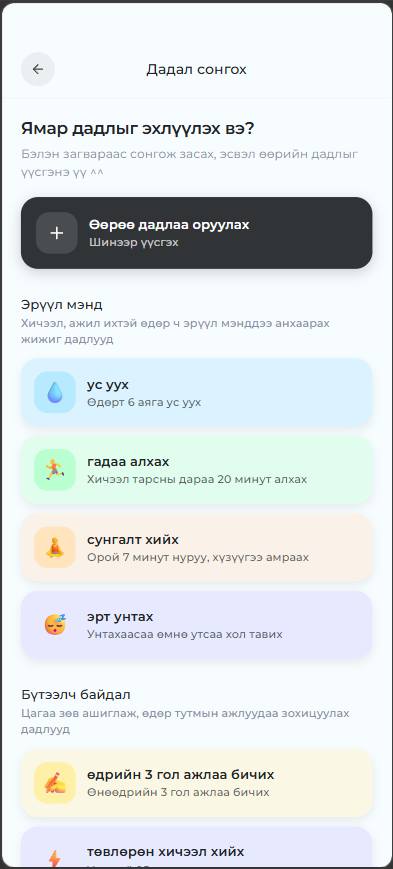
\includegraphics[width=\textwidth,height=0.46\textheight,keepaspectratio]{images/frontend/addhabit.png}
    \\[4pt]\small (а) Дадлын нэр, хэлбэр, хуваарийн тохиргоо
  \end{minipage}
  \hfill
  \begin{minipage}[b]{0.42\textwidth}
    \centering
    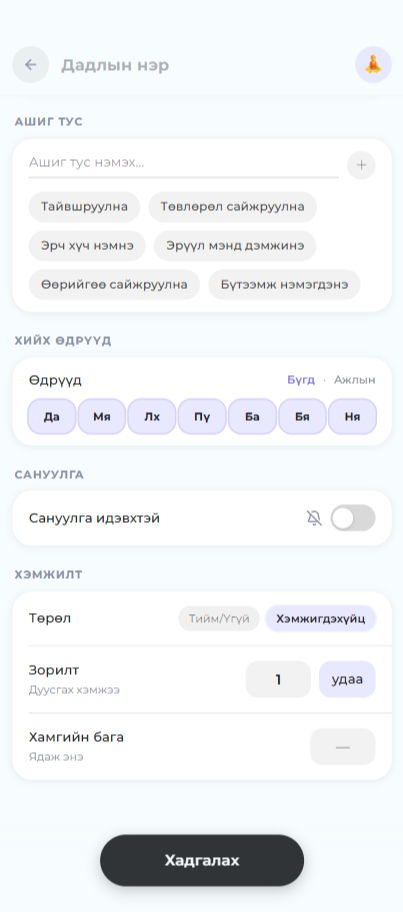
\includegraphics[width=\textwidth,height=0.46\textheight,keepaspectratio]{images/frontend/addhabit2.png}
    \\[4pt]\small (б) Сануулга болон хэмжилтийн тохиргоо
  \end{minipage}
  \caption{Дадал үүсгэх дэлгэц}
  \label{fig:addhabit}
\end{figure}

\subsection{Хурдан бүртгэлийн дэлгэц}

Дашборд дэлгэцийн дадлын картан дээрх `\texttt{+}' товчийг дарахад bottom sheet хэлбэрийн хурдан бүртгэлийн дэлгэц нэмэлтгүй нуугдана. Хэрэглэгч тоон keyboard-оор бодит гүйцэтгэлийн утгаа оруулахад систем зорилтын хязгаарыг шалгаж, зорилт биелсэн тохиолдолд тэмдэглэгдсэн баталгааг харуулна (Зураг~\ref{fig:quicklog}).

\begin{figure}[htbp]
  \centering
  \begin{minipage}[b]{0.42\textwidth}
    \centering
    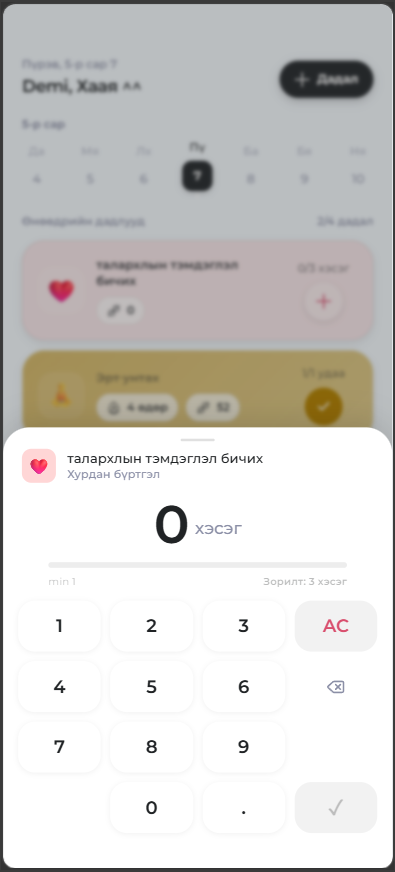
\includegraphics[width=\textwidth,height=0.46\textheight,keepaspectratio]{images/frontend/habitBurtgel.png}
    \\[4pt]\small (а) Утга оруулах байдал
  \end{minipage}
  \hfill
  \begin{minipage}[b]{0.42\textwidth}
    \centering
    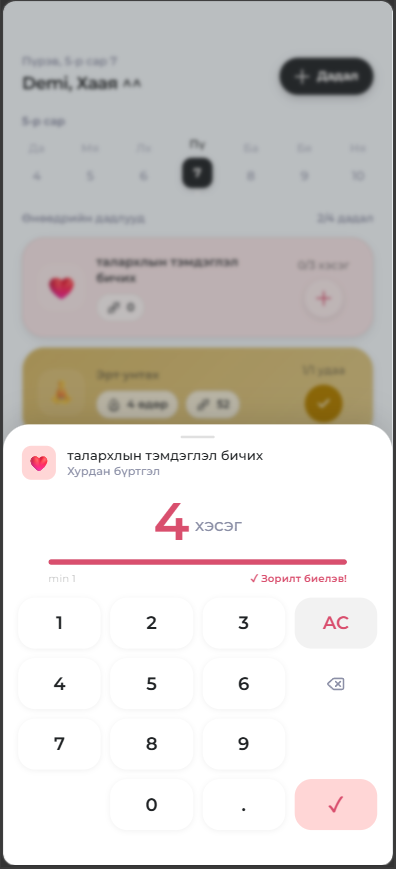
\includegraphics[width=\textwidth,height=0.46\textheight,keepaspectratio]{images/frontend/habitBurtgel2.png}
    \\[4pt]\small (б) Зорилт биелэсэн баталгааны дэлгэц
  \end{minipage}
  \caption{Хурдан бүртгэлийн дэлгэц}
  \label{fig:quicklog}
\end{figure}

\subsection{Ахицын шинжилгээний дэлгэц}

Ахицын дэлгэц нь нийт болон дадал бүрийн байдлаар шүүх боломжтой сарын calendar хуанли болон дадлын хүчний дугуй диаграммыг агуулна. Дадлын хүчний оноо, одоогийн болон шилдэг streak, нийт гүйцэтгэлийн тоо, өдрийн дундаж, мөн сүүлийн эргэцүүллийн тэмдэглэлүүдийг нэг дэлгэцэд нэгтгэн харуулдаг (Зураг~\ref{fig:analytics}).

\begin{figure}[htbp]
  \centering
  \begin{minipage}[b]{0.30\textwidth}
    \centering
    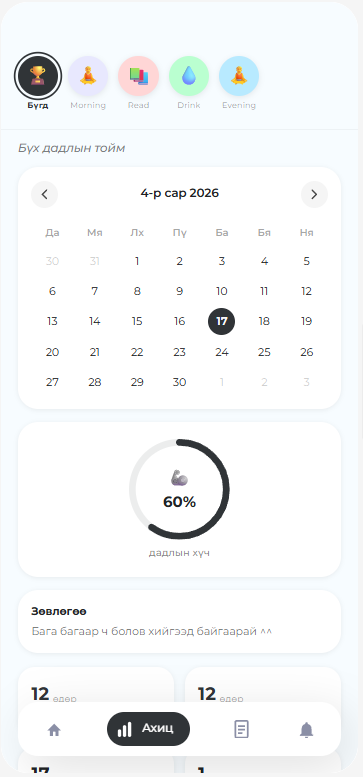
\includegraphics[width=\textwidth,height=0.34\textheight,keepaspectratio]{images/frontend/analytics.png}
    \\[4pt]\small (а) Бүх дадлын нэгдсэн тойм
  \end{minipage}
  \hfill
  \begin{minipage}[b]{0.30\textwidth}
    \centering
    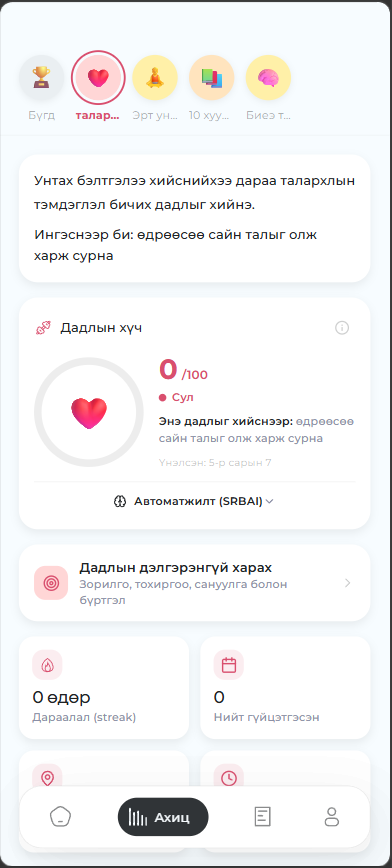
\includegraphics[width=\textwidth,height=0.34\textheight,keepaspectratio]{images/frontend/analytics2.png}
    \\[4pt]\small (б) Тухайн дадлын calendar болон хүчний оноо
  \end{minipage}
  \hfill
  \begin{minipage}[b]{0.30\textwidth}
    \centering
    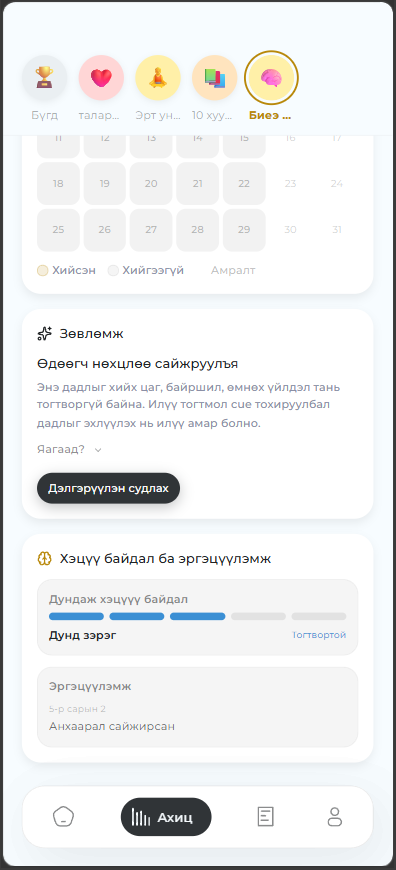
\includegraphics[width=\textwidth,height=0.34\textheight,keepaspectratio]{images/frontend/analytics3.png}
    \\[4pt]\small (в) Streak, статистик, эргэцүүлэл
  \end{minipage}
  \caption{Ахицын шинжилгээний дэлгэц}
  \label{fig:analytics}
\end{figure}

\subsection{Суралцах агуулгын дэлгэц}

Суралцах (Learn) дэлгэц нь хэрэглэгчид дадал хэвшүүлэлтийн онолын үндэслэлийг уншиж судлах боломж олгодог. Нийтлэлүүд ``Танд зориулсан'', ``Бүтээлч байдал'', ``Эрүүл мэнд'', ``Сэтгэлгээ'' гэсэн 4 ангилалд хуваагдаж, 3 минутын уншлагаар тухайн сэдвийг тайлбарладаг (Зураг~\ref{fig:learn}).

\begin{figure}[htbp]
  \centering
  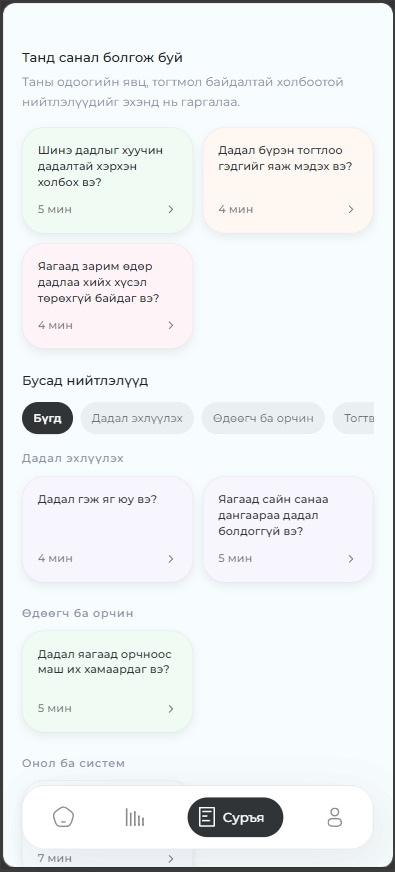
\includegraphics[width=0.42\textwidth,height=0.46\textheight,keepaspectratio]{images/frontend/learn.png}
  \caption{Суралцах агуулгын дэлгэц}
  \label{fig:learn}
\end{figure}

\subsection{Профайл, санал хүсэлт ба судалгааны хэсэг}

Profile дэлгэц нь хэрэглэгчийн ерөнхий төлөв болон системийн нэмэлт тохиргоог нэг дор төвлөрүүлсэн. Энэ хэсэгт идэвхтэй дадлын тоо, нээсэн амжилт, нийт XP, push notification-ийн зөвшөөрөл, архивласан дадлууд, theme сонголт, санал хүсэлт, нууц үг солих, заавар дахин харах зэрэг боломжуудыг оруулсан.

Системийг 20 хэрэглэгчээр туршуулах үе шатанд хэрэглэгчийн чанарын болон тоон үнэлгээг авах шаардлагатай болсон тул profile хэсэгт Google Forms судалгааны холбоосыг тусдаа ``Судалгаа'' карт хэлбэрээр байршуулсан. Ингэснээр хэрэглэгч системийг ашигласныхаа дараа апп дотроос шууд судалгаа бөглөж, ашиглахад хялбар байдал, сануулгын үр нөлөө, ахицын мэдээллийн хэрэгцээ, сайжруулах санал зэргийг илгээх боломж бүрдсэн.

\subsection{API клиент}

Фронтэнд талын \texttt{api/client.ts} нь суурь HTTP клиентийг агуулж, хэрэглэгчийн JWT токеныг Authorization header-д автоматаар хавсаргана. Хэрэв 401 алдаа ирвэл хэрэглэгчийг дахин нэвтрэх урсгал руу шилжүүлдэг. API функцуудыг \texttt{auth}, \texttt{habits}, \texttt{progress}, \texttt{reminders}, \texttt{push}, \texttt{engagement}, \texttt{learning} зэрэг тусдаа файлуудад хувааснаар дэлгэцүүд серверийн endpoint-уудтай нэг мөрийн интерфэйсээр харилцах боломжтой болсон.

\renewcommand{\arraystretch}{1.15}
\setlength{\LTpre}{0pt}
\setlength{\LTpost}{0pt}

\begin{longtable}{L{1.5cm}L{8.4cm}L{4.0cm}}
\caption{Системийн үндсэн API endpoint-ууд}
\label{tab:api-overview}\\

\toprule
\textbf{Method} & \textbf{Path} & \textbf{Зорилго} \\
\midrule
\endfirsthead

\multicolumn{3}{c}{\textit{Хүснэгт \thetable\ үргэлжлэл}}\\
\toprule
\textbf{Method} & \textbf{Path} & \textbf{Зорилго} \\
\midrule
\endhead

\midrule
\multicolumn{3}{r}{\textit{Дараагийн хуудсанд үргэлжилнэ}}\\
\endfoot

\bottomrule
\endlastfoot

POST  & \nolinkurl{/auth/register} & Шинэ хэрэглэгч бүртгэх \\
POST  & \nolinkurl{/auth/login} & Нэвтрэх, JWT токен авах \\

POST  & \nolinkurl{/users/:userId/habits} & Дадал үүсгэх \\
GET   & \nolinkurl{/users/:userId/habits} & Дадлын жагсаалт авах \\
GET   & \nolinkurl{/users/:userId/habits/today} & Өнөөдрийн хуваарьт дадлуудыг авах \\
GET   & \nolinkurl{/users/:userId/habits/:habitId} & Нэг дадлын дэлгэрэнгүй мэдээлэл авах \\
PATCH & \nolinkurl{/users/:userId/habits/:habitId} & Дадал засах, архивлах \\

POST  & \nolinkurl{/users/:userId/habits/:habitId/logs} & Гүйцэтгэл бүртгэх \\
GET   & \nolinkurl{/users/:userId/habits/:habitId/logs} & Гүйцэтгэлийн бүртгэлийн түүх авах \\
PATCH & \nolinkurl{/users/:userId/habits/:habitId/logs/:logId} & Гүйцэтгэлийн утгыг засах \\
GET   & \nolinkurl{/users/:userId/habits/:habitId/progress-summary} & Ахицын нэгдсэн тойм авах \\
POST  & \nolinkurl{/users/:userId/habits/:habitId/logs/:logId/difficulty} & Төвөгшлийн үнэлгээ оруулах \\
POST  & \nolinkurl{/users/:userId/habits/:habitId/logs/:logId/reflection} & Эргэцүүллийн тэмдэглэл оруулах \\
GET   & \nolinkurl{/users/:userId/habits/:habitId/adaptation-recommendation} & Дасан зохицох зөвлөмж авах \\
POST  & \nolinkurl{/users/:userId/habits/:habitId/srbai-assessments} & SRBAI үнэлгээ оруулах \\
GET   & \nolinkurl{/users/:userId/habits/:habitId/habit-strength/composite} & Нийлмэл дадлын хүчний оноо авах \\

POST  & \nolinkurl{/users/:userId/habits/:habitId/reminders/evaluate-and-create} & Сануулгыг үнэлж үүсгэх \\
GET   & \nolinkurl{/users/:userId/reminders} & Хэрэглэгчийн сануулгын жагсаалт авах \\
POST  & \nolinkurl{/users/:userId/reminders/:reminderId/actions} & Сануулгад өгсөн үйлдлийг бүртгэх \\
POST  & \nolinkurl{/users/:userId/habits/:habitId/reminder-policy/apply-tapering} & Сануулгын бодлогын шинэчлэл хэрэглэх \\

GET   & \nolinkurl{/users/:userId/push-subscriptions} & Push subscription жагсаалт авах \\
POST  & \nolinkurl{/users/:userId/push-subscriptions} & Төхөөрөмжийн push subscription бүртгэх \\
DELETE & \nolinkurl{/users/:userId/push-subscriptions/:subscriptionId} & Push subscription устгах \\
POST  & \nolinkurl{/admin/push/broadcast} & Нийт хэрэглэгчдэд push мэдэгдэл илгээх \\

GET   & \nolinkurl{/users/:userId/engagement/summary} & XP, badge, achievement-ийн нэгдсэн мэдээлэл авах \\
POST  & \nolinkurl{/users/:userId/feedback} & Аппын санал хүсэлт илгээх \\
GET   & \nolinkurl{/users/:userId/recommendations} & Дасан зохицох зөвлөмжийн жагсаалт авах \\
GET   & \nolinkurl{/users/:userId/articles} & Суралцах нийтлэлүүд авах \\
POST  & \nolinkurl{/users/:userId/activity-logs} & Ерөнхий хэрэглээний идэвхийн лог бүртгэх \\

\end{longtable}

\section{Бүлгийн дүгнэлт}

Энэ бүлэгт зан үйлд суурилсан дадал хэвшүүлэх системийн эцсийн хэрэгжүүлэлтийг тайлбарлав. Үүнд технологийн стек, кодын сангийн бүтэц, өгөгдлийн сангийн хэрэгжилт, сануулгын шийдвэрийн дүрэм, дадлын хүчний тооцоолол, дасан зохицох зөвлөмж, push notification, engagement буюу урамшууллын модуль, бэкэнд болон фронтэндийн үндсэн дэлгэцүүд, API-ийн зохион байгуулалт зэргийг авч үзлээ.

Хэрэгжүүлэлтийн үр дүнд хэрэглэгчийн бүртгэл, дадал үүсгэх/засах, олон цагийн хүрээ болон cue тохируулах, гүйцэтгэл бүртгэх, сануулга илгээх, SRBAI үнэлгээ авах, дадлын хүч тооцоолох, ахицын мэдээлэл боловсруулах, зөвлөмж гаргах, XP болон badge олгох, санал хүсэлт авах, судалгаанд чиглүүлэх зэрэг системийн үндсэн болон нэмэлт боломжууд ажиллах түвшинд хүрсэн. Мөн \texttt{ReminderDecisionRules}, \texttt{HabitStrengthRules}, \texttt{AdaptationRules} зэрэг зан үйлийн дэмжлэгийн дүрмүүдийг бодит кодын түвшинд хэрэгжүүлснээр өмнөх бүлгүүдэд боловсруулсан онолын загварыг хэрэглэгчдээр туршуулах боломжтой програм хангамжийн бүрэн шийдэл болгон буулгасан.

